\documentclass[10pt]{article}
\usepackage[T1]{fontenc}
\usepackage{lmodern,amsmath,amssymb,graphicx,hyperref}
\usepackage[margin=.74in]{geometry}
\setlength{\parindent}{0pt}\setlength{\parskip}{6pt}
\begin{document}
\begin{center}{\Large Uniform multiplicity and the known target sign}\\[4pt]
17 November2026 --- local unsigned Lean evidence\end{center}
\textbf{Full mixed multiplicity, without factorials.} Write the actual
bivariate polynomial as $p(X,Y)=\sum_j p_j(X)Y^j$. Define
\[
 J_{x,t}(Y)=\sum_j [T^t]p_j(T+x)\,Y^j.
\]
The local condition at $(x,y)$ requires every coefficient
$[U^k]J_{x,t}(U+y)$ to vanish whenever $t+k<r$. It therefore includes
all mixed Taylor coefficients, not just one directional derivative.
Source011 derives its $r=1$ evaluation equivalence and
\[
 (Y-y)^{r-t}\mid J_{x,t}(Y)\quad(0\le t<r).
\]
The proof divides by no factorials and permits $r$ above the odd characteristic
[pcc:unverified].

\textbf{Actual all-uniform-multiplicity result.} Let $a\ge2$, let $S$ contain
$2a$ distinct abscissas, assume $2\ne0$ and $z(x)\ne0$, and impose the same
full multiplicity $r$ at \emph{both} $(x,z(x))$ and $(x,-z(x))$ for every
$x\in S$. Homogenize to degree $\ell\ge d=\deg_Yp$ and use the exact strict
natural coefficient budget
\[
 \deg p_j+ja+(\ell-j)(a-2)<2ar.
\]
Then $p=0$, for every uniform $r$ and homogeneous degree $\ell$. The field
statement applies to prime fields satisfying its explicit conditions; it
is not a conclusion about all ECDLP algorithms [pcc:unverified].

\textbf{Readable proof.} Suppose $p\ne0$ and let $d=\deg_Yp$.
The leading coefficient and strict budget give $d<2r$. Put
$s=r-\lfloor d/2\rfloor>0$. For $t<s$, each $J_{x,t}$ has degree at most $d$
but is divisible by two coprime linear powers of total degree $2(r-t)>d$.
Thus $J_{x,t}=0$. The actual leading coefficient $p_d$ consequently has
multiplicity at least $s$ at all support abscissas:
\[
 \left(\prod_{x\in S}(X-x)\right)^s\mid p_d,
 \qquad \deg p_d\ge2as.
\]
Its weighted contribution satisfies
\[
 \deg p_d+ad+(\ell-d)(a-2)\ge a(2s+d)\ge2ar,
\]
contradicting strictness. Existing univariate divisor and degree laws supply
the proof; the proposed multivariate cancellation induction is not used
[pcc:unverified].

\textbf{Evidence.} Source011, build012, receipt006,
PCC-20261117-3bcc1a:36 source statements including29 parent and7 new.
Accepted exit0/no warnings and standard printed foundations.
\newpage
\begin{center}{\Large The target sign changes the actual input}\end{center}
\textbf{Singleton target control.} A public target has a known ordinate,
so only its chosen sign need appear in its list. Source013 checks this changed
hypothesis at multiplicity \emph{one}: the target has one branch, the other
$2a-1$ abscissas retain both signs. The same strict budget implies
\[
 \deg_Yp\le1,\qquad \deg p_0<2a,\qquad \deg p_1<a.
\]
Paired constraints off target force $p_1$ to vanish at $2a-1$ abscissas, hence
$p_1=0$. The chosen branch at all $2a$ abscissas then forces $p_0=0$.
No negative-target constraint was added. This is not an all-multiplicity
singleton-target theorem [pcc:unverified].

\textbf{The primary sufficient count condition.} Suppose $u$ of the $2a$
positions have unresolved two-branch lists and the rest are fixed singletons.
There are $2a+u$ interpolation points and target agreement $2a$.
Substitution into Beelen et al2013, SectionIII/Theorem6, condition(2), gives
these twice-counts:
\[
 V_2=2(\ell+1)\bigl(2ar-(a-1)\ell\bigr),\qquad
 C_2=(2a+u)r(r+1).
\]
Its sufficient admission requires $C_2<V_2$. Source014 establishes
$V_2<C_2$ whenever $a\ge3$, $u\ge3$, $r\ge1$ and $\ell$ is an integer.
In particular this covers the count criterion with only the target fixed,
$u=2a-1$ [pcc:unverified].

The exact certificate is
\begin{align*}
 C_2-V_2={}&(2\ell-3r+1)^2+(3r-1)\\
 &+2(a-3)(\ell-r)(\ell-r+1)+(u-3)r(r+1)>0.
\end{align*}
The product of consecutive integers is nonnegative even when
$\ell-r<0$. The other terms have the stated signs [pcc:unverified].

\textbf{Positive control, with a genuinely changed regime.}
For $a=2$, $u=3$, $r=4$, $\ell=7$, the criterion gives
\[
 V_2/2=72>70=C_2/2.
\]
Here $a=2$ means four support positions on the prime-field curve, not field
characteristic two. This checks parameter arithmetic. The actual coefficient
operator has not yet been constructed; no relation, scalar or growing-family
algorithm is claimed [pcc:unverified].

\textbf{Necessary distinctions.} $V_2$ is the primary coefficient lower
count when ranges clip; failure of this sufficient condition is not
nonexistence of rank-dependent helpers. The all-uniform theorem on page1,
the singleton multiplicity-one theorem and this arithmetic admission test
are three different results. Published fast interpolation with one Lagrange
ordinate per abscissa is not automatically a method or cost bound for
repeated-abscissa two-branch lists.
\newpage
\begin{center}{\Large Evidence and the next public construction}\end{center}
\begin{center}
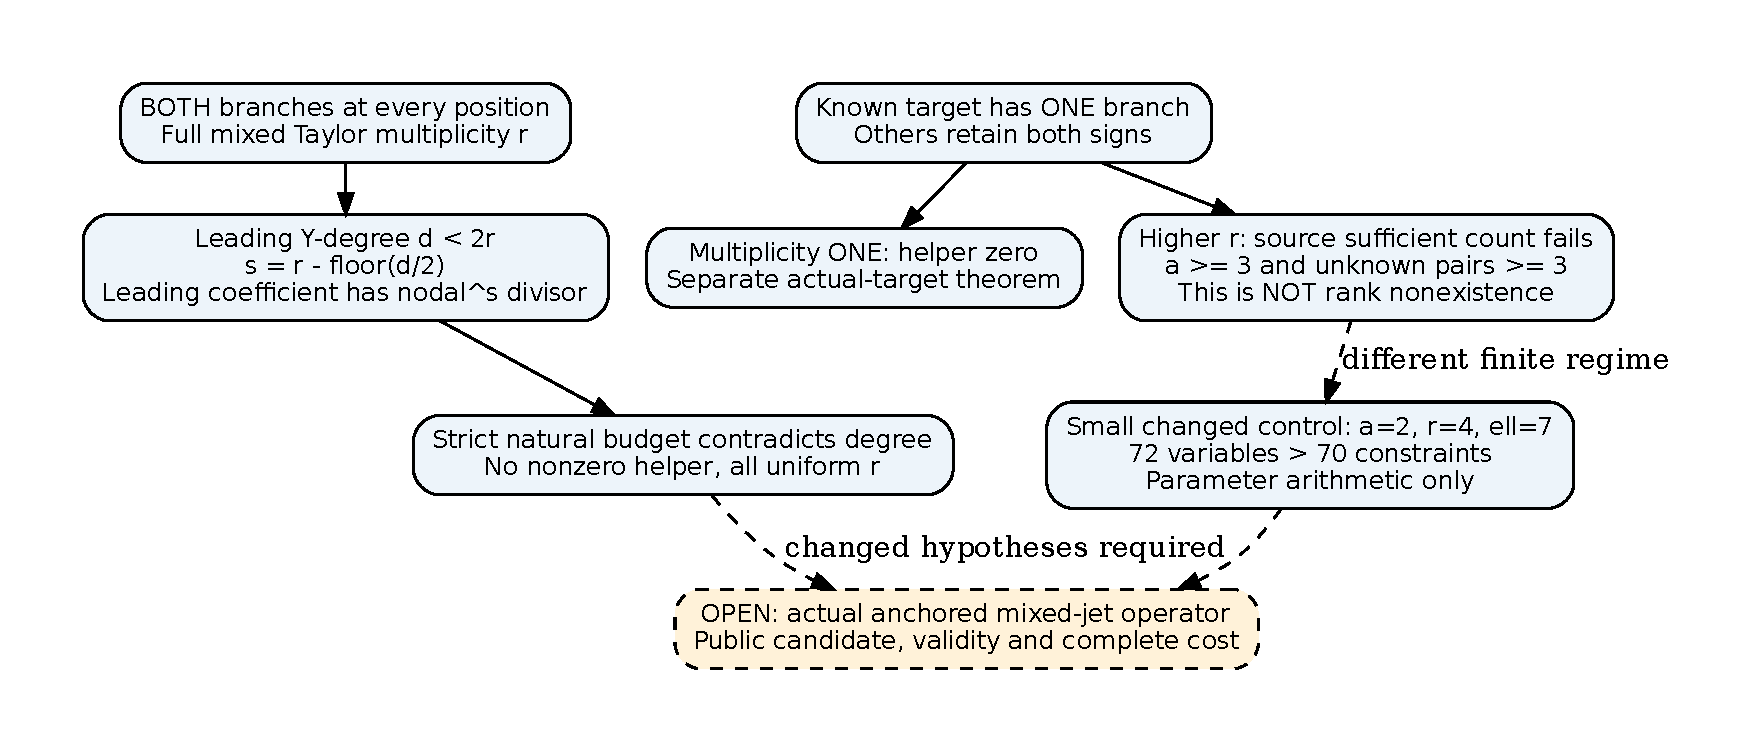
\includegraphics[width=.93\linewidth,height=3.65in,keepaspectratio]{uniform-dependencies-001.pdf}
\end{center}
\textbf{Exact proof map.} Instances006--008 bind definitions and hypotheses.
Source011/build012/receipt006 has7 new statements;
source013/build014/receipt007 has2 more, PCC-20261117-bb5895;
source014/build015/receipt008 has3 more, PCC-20261117-896a0c.
Final source41 includes29 parent plus12 new statements, not41 new ones.
Every accepted build exits0 without warnings; all41 final dependency prints
are standard. These are local unsigned producer records, default
\texttt{not\_covered}, outside shared Transport53/57 audit/fresh
[pcc:unverified].

\textbf{What is next.} Construct the anchored public coefficient-to-full-jet
linear operator with actual repeated-abscissa constraints and finite
coefficient encoding. First bind the72-to70 control to actual coefficients
and mixed Taylor conditions without successful signs supplied as input.
Then distinguish auxiliary generation, factor/root output, valid full norm,
useful target-scalar relation and complete expected bit cost. For growing
$a$, a nonzero kernel needs actual structure or evidence; it cannot be assumed
from the failed sufficient-count test.

\textbf{Preservation and sources.} All accepted, failed and warning sources
and raw logs remain beside the report. No old immutable artifact or claim
was overwritten; no native, paid, attack, timing or scaling campaign ran.
Prior canonical scoreboards are unchanged because there is no measured
speed result. The same protected provenance blocker prevents publication;
no ledger rewrite, forcepush or automation edit was used.

Primary reference:
\href{https://doi.org/10.1109/TIT.2013.2243800}{Beelen, H\o holdt, Nielsen and Wu (2013), Theorem6/(2)}.
Read scope is retained in literature-review001/PCC-20261117-4bcf3a.
Existing Mathlib Polynomial OfFn, AlgebraMap, Div, Coprime, Roots and
Lagrange laws are used as stated. KB unavailable; no novelty claim.
Next exact scope is \texttt{PROTOCOL-002.md} and versioned continuation012.
The optional anchored cubic/norm sketch remains unvalidated.
\end{document}
